\section{Следствие из теоремы Эйлера о связи числа вершин, ребер и граней в плоском графе.  Доказать, 
что для графов - триангуляций выполняется верхняя оценка следствия.}

Теорема Эйлера справедлива для любых псевдографов, следствие из нее
справедливо только для простых графов.

\textbf{Следствие:}
Если связный простой плоский граф имеет $n$ вершин, где $n \geq 3$ и
$r$ ребер то справедливо неравенство: $3n - r \geq 6$.

\begin{proof}
    Обозначим через qk число граней, ограниченных k ребрами.
    Так как в графе нет петель и кратных ребер, то $q_1 = q_2 = 0$. Поэтому число всех
    граней равно: $q = q_3 + q_4 + \dots$.

    Покажем, что справедливо равенство $2r = 3q_3 + 4q_4 + \dots$.

    В нем справа найдено количество всех ребер, ограничивающих каждую
    грань. Так, q3 – количество граней, ограниченных 3 ребрами, поэтому $3q_3$ --
    количество всех ребер, ограничивающих эти грани. Каждое ребро в этой
    сумме учитывается дважды, так как каждое ребро принадлежит двум граням
    (или два раза одной грани), поэтому слева стоит множитель 2.
    Получаем: $2r = 3q_3 + 4q_4 + \dots \geq 3(q_3 + q_4 + \dots) = 3q$.
    Поэтому $2r \geq 3q$, поэтому $q \geq \frac{2}{3}r$.

    По теореме Эйлера $n-r+q=2$. Тогда $q = 2 - n + r \geq \frac{2}{3}r$.

    $6 - 3n + 3r - 2r \geq 0$, поэтому получаем: $3n - r \geq 6$.
\end{proof}

В следствии доказывается, что если связный плоский граф имеет
$n$ вершин, где $n \geq 3$ и $r$ рёбер, то справедливо неравенство: $3n - r \geq 6$.

В связи с этим возникает вопрос: существуют ли графы с верхней оценкой,
то есть для любого ли n существует планарный граф, для которого верно
$3n - r = 6$. Оказывается, существуют.

\begin{definition}
    Это связные планарные графы, в которых любая грань (включая внешнюю)
    ограничена циклом длины 3. Такие графы называются \textit{триангуляциями}.
\end{definition}

\newpage
Докажем методом математической индукции по числу вершин $n$, где $n \geq 3$,
что для таких графов равенство $3n - r = 6$ выполняется.

\begin{enumerate}[left=0.0em, labelsep=1em, topsep=0.0em, itemsep=0pt, parsep=0.5em]
    \item Если $n=3$, то таким графом является полный граф $К_3$. Для него $9-3 =6$.
    \item Пусть для n у такого графа равенство выполняется: $3n - r =6$. Докажем,
    что для такого графа с $n+1$ вершиной равенство также будет
    выполняться.
    К имеющемуся графу с $n$ вершинами добавляем одну вершину. Она
    попадет в один из треугольников. Соединяем ее с тремя вершинами
    треугольника, внутрь которого она попала, при этом планарность не
    нарушается. Таким образом, добавляется 3 ребра, то есть у графа $(n+1)$
    вершина и $(r+3)$ ребра.
    \begin{align*}
        3(n+1) - (r+3) = 3n + 3 - r - 3 = 3n - r =6.
    \end{align*}
    \item По методу математической индукции заключаем, что равенство
    справедливо для любого $n$.
\end{enumerate}

\textbf{Пример:} Для графа на рисунке удостовериться, что справедлива формула
Эйлера, равенство $2r = 3q_3 + 4q_4 + \dots$ и неравенство $3n - r \geq 6$.
\begin{figure}[h]
    \centering
    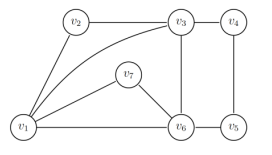
\includegraphics[scale=0.5]{31.png}
\end{figure}

$n=7, r = 10, q=5. 7-10+5 =2$ (верно)\\
$q_3 =2, q_4 = 2, q_6 = 1$ (внешняя грань)\\
$20 = 3 \cdot 2+ 4 \cdot 2 + 6 \cdot 1 = 6+8+6$ (верно)\\
$3 \cdot 7 - 10 \geq 6$ (верно)